\documentclass{llncs}

\usepackage{amssymb}
\setcounter{tocdepth}{3}
\usepackage{graphicx}
\usepackage[table,xcdraw]{xcolor}
\usepackage[ruled]{algorithm2e}
%\usepackage[lined,boxed,commentsnumbered]{algorithm2e}
\usepackage{amssymb}
\usepackage{amsmath,graphicx,color,doi}
\usepackage{algorithm2e}
%\usepackage{algorithmic}	
\usepackage{multirow}
\usepackage{subfigure}
\usepackage{cite}


\newcommand{\gi}[1]{{\textcolor{red}{[\small \textbf{Giacomo}: #1]}}}
\newcommand{\ad}[1]{{\textcolor{red}{[\small \textbf{Adriano}: #1]}}}
\newcommand{\cl}[1]{{\textcolor{red}{[\small \textbf{Claudio}: #1]}}}

%\newcommand{\gi}[1]{}
%\newcommand{\ad}[1]{}
%\newcommand{\cl}[1]{}


\begin{document}
\title{Tampering Detection In Low-Power Smart Cameras}

\author{Adriano Gaibotti\inst{1} \and Claudio Marchisio\inst{1} \and Alexandro Sentinelli\inst{1} \and Giacomo Boracchi\inst{2}}

\institute{ 
	STMicroelectronics, Advanced System Technology, Via Camillo Olivetti 2, 20864, Agrate Brianza (MB), Italy\\
	\email{\{adriano.gaibotti, claudio.marchisio, alexandro.sentinelli\}@st.com}
	\and
	Politecnico di Milano, Dipartimento di Elettronica, Informazione e Bioingegneria (DEIB), Via Ponzio 34/5, 20133, Milano (MI), Italy\\
	\email{giacomo.boracchi@polimi.it}
}
\maketitle

\begin{abstract}
A desirable feature for smart cameras is the ability to autonomously detect any tampering event/attack that would prevent a clear view over the monitored scene. No matter whether tampering is due to atmospheric phenomena (e.g., few rain drops over the camera lens) or to malicious attacks (e.g., the device displacement), these have to be promptly detected to possibly activate countermeasures. Tampering detection becomes particularly challenging in battery-powered cameras, where it is not possible to acquire images at video-like frame-rates, nor use sophisticated image-analysis algorithms. 

We here introduce a tampering-detection algorithm specifically designed for low-power smart cameras: the algorithm leverages very simple indicators that are then monitored by an outlier-detection scheme. Any frame yielding anomalous indicator is detected as a tampering attempt. Core of the algorithm is the partitioning of the scene into adaptively defined regions, that are preliminarily defined by segmenting the image during the algorithm-configuration phase, and which shows to substantially improve the detection of camera displacements. Our experiments show that the proposed algorithm can successfully operate on sequences acquired at very low-frame rate, such as one frame every minute, with a very small computational complexity. %and leveraging the image partitioning into regions yields improved performance with respect to monitoring the whole scene


\keywords{tampering detection, defocus, displacement detection}
\end{abstract}



\section{Introduction}\label{sec:introduction}
%\gi{Adriano: decidi che email tenere, non tutte e due :)}

%We here address the problem of detecting tampering events/attacks in camera devices, and in particular those preventing the proper acquisition of the monitored scene. 

% What is the problem?
When cameras operate outdoor and in harsh environments, dust, rain drops or snow flakes might lie on the camera lens resulting in blurry pictures, as in Fig. \ref{fig:pioggia}, or in partial occlusions of the scene, as in Fig. \ref{fig:neve}. Similarly, intentional attacks like displacing the camera, changing its focus, or spraying some opaque or glossy liquid over the lenses, would result in heavily compromised pictures, that would be surely useless for monitoring purposes. We refer to these events/attacks as tampering. In some cases, tampering is easy to detect, e.g., when the camera integrity is affected and the device goes out-of-order. However, in many other situations, namely when the device is not physically damaged, tampering detection is not straightforward, and sometimes image analysis is the only viable option. 

\begin{figure}[t!]
\centering
\subfigure[]{\label{fig:pioggia} 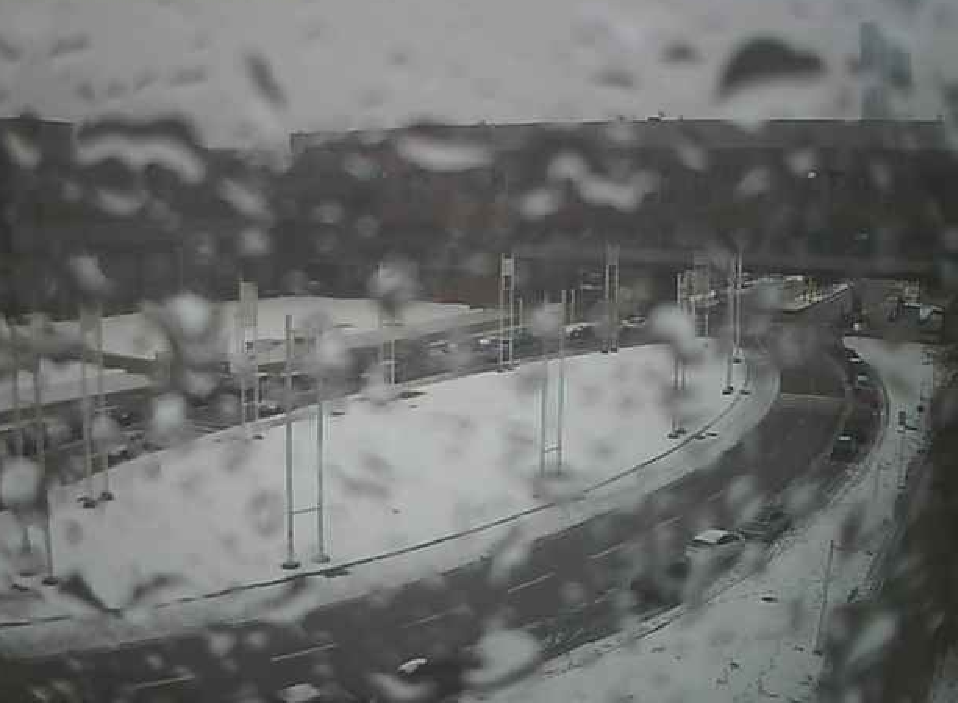
\includegraphics[width=0.4\linewidth]{Immagini/pioggia}}
\subfigure[]{\label{fig:neve} 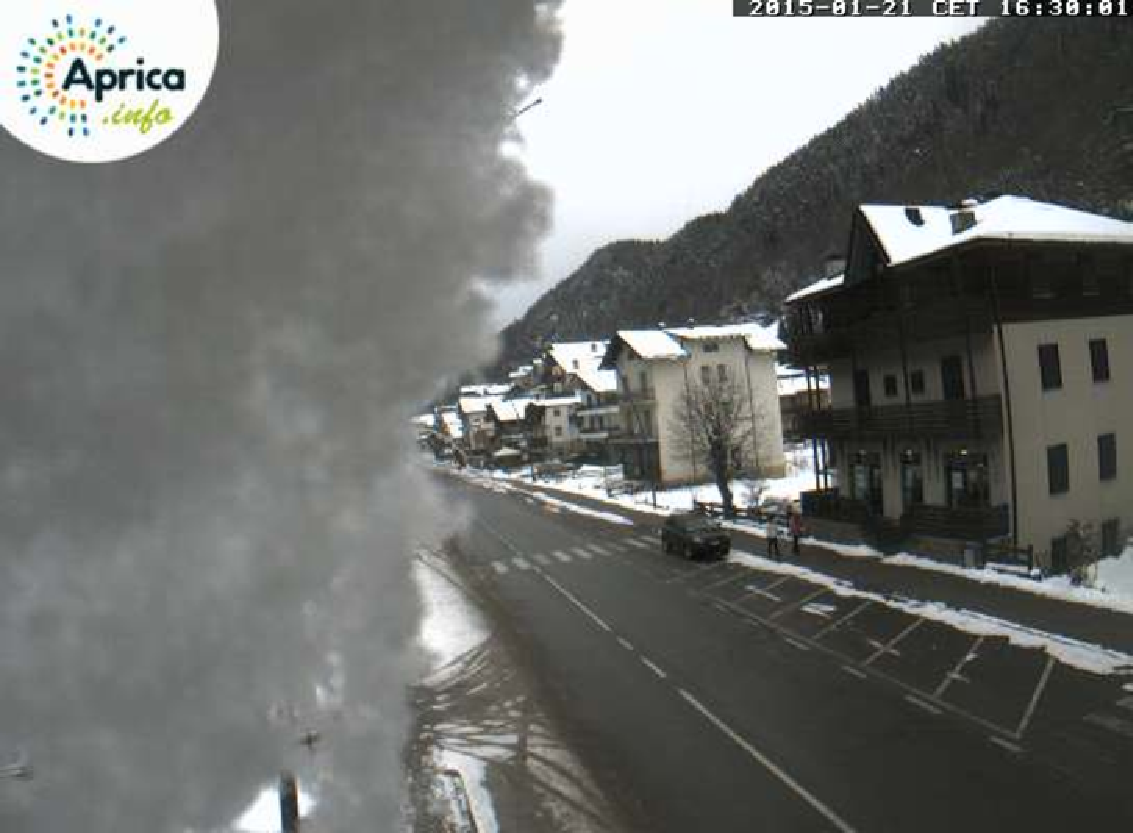
\includegraphics[width=0.4\linewidth]{Immagini/neve}}
\caption[Tampering examples]{Examples of tampering events due to atmospheric phenomena. \textbf{(a)} Blur due to rain drops on the camera lens. \textbf{(b)} Occlusion due to snow on the camera lens.}
\label{fig:tampering}
\end{figure}

% Why is it interesting and important?
Tampering detection is an essential feature in surveillance systems~\cite{hampapur2005smart}, where cameras are expected to autonomously detect any tampering, and promptly reporting alerts. In fact, tampering prevents the correct scene interpretation: even a mild blur might result in important details such as licence plates. Surveillance cameras are typically connected to the power supply and operates at normal frame-rates (e.g. around few frames per second): in these conditions, several tampering-detection algorithms have been presented~\cite{TODO}.  

In this work we expressly target low-power and ultra-low-power smart cameras\gi{una reference qua ci vuole}, battery-powered devices that are characterized by a constrained computational power and memory availability. Even though these devices are not meant for critical surveillance applications, they are becoming popular in distributed systems for monitoring wide environments due to their low cost and maintenance requirements.  %As an example, consider Wireless Multimedia Sensor Networks (WMSN) \cite{akyildiz2007survey} where smart-cameras can acquire and transmit images at regular time interval or upon requests. 
% These units are not connected to the power supply and have to operate with batteries and possibly rely on energy harvesting~\cite{magno2009adaptive}. 
%In practice, because of energy constrain, low-power devices have to operate at very low frame-rates: possibly less than one frame every minute.  

% Why is it hard? (E.g., why do naive approaches fail?)
Tampering detection in low-power smart cameras has not been much investigated in the literature~\cite{alippi2010detecting} while being more challenging than in conventional surveillance cameras~\cite{perrig2004security}. Beside computational aspects -- such as the number of operations per pixels allowed -- the big issue is that low-power smart cameras typically operate at very low-frame rates (e.g., less than one frame per minute), thus the acquired sequence does not evolve smoothly. This prevents the use of learned background models and the analysis of foreground variations \cite{piccardi2004background}. In fact, when dynamic environments are acquired at low frame rates, two consecutive frames might be very different because of changes in the scene and in the light conditions, yielding sequences like those in Figure~\ref{fig:sequences}. Smart cameras have to promptly distinguish between \emph{normal} scene or illumination changes, and changes due to camera tampering to avoid the transmission of corrupted frames. Moreover, the false-alarm rate is a serious concern, a any false alarm results in wasting energy for data processing and network transmissions.
% We here address the problem of detecting tampering events on a camera device that is employed for monitoring purpose. Tampering events can be due to malicious attacks, as for instance a displacement of the camera or spraying some dirty liquid that would prevent the acquisition of (part of) the monitored scene or the interpretation of the content (e.g., the identification of licence plates). 

%What are the key components of my approach and results? Also include any specific limitations.
We here address the detection of camera blurring and displacement, which are presented in Section \ref{sec:probForm}. The proposed algorithm, detailed in Section~\ref{sec:propSol}, relies on two indicators: the average image intensity to detect displacement, and the average gradient norm, to detect blurring. These indicators can be easily computed and monitored by an outlier-detection technique in a low-power smart camera, thus our solution is meant as a very prompt trigger to be possibly combined with other sequential monitoring techniques. In particular, we show that separately monitoring the indicators over different regions of the scene can substantially improve the displacement-detection performance. Remarkably, these regions can be preliminarily defined during an initial configuration phase (Section \ref{subsec:Segmentation}), thus the algorithm operates at a negligible computational overhead w.r.t. monitoring the whole image. Experiments in Section \ref{sec:experiments} show that leveraging image regions can substantially improve the displacement-detection performance. % Concluding remarks and discussions are given in Section \ref{sec:Conclusion}.


\subsection{Related Works}\label{subsec:relWorks}
% Why hasn't it been solved before? (Or, what's wrong with previous proposed solutions? How does mine differ?)
The literature concerning tampering detection is mostly focused on video surveillance applications and operates at few frames per second \gi{Adriano, \'e vero?}. Background models are typically leveraged to identify defocus and occlusions; in particular~\cite{aksay2007camera} performs defocus detection by analyzing the wavelet domain of each frame and performs histogram comparison for detecting occlusions, while camera displacements are not considered. A background-subtraction technique is employed in~\cite{saglam2009real} to identify defocus, occlusions, and displacements. \gi{FIXME Comparison in the Fourier domain for defocus detection, histogram comparison for occlusion detection, comparison between current background and delayed background for displacement detection}. Background subtraction is also used in \cite{gil2007automatic} to detect defocus, occlusions, and displacements. \gi{FIXME Comparison of edges pixels count for defocus detection, entropy comparison for occlusion detection, block matching algorithm for displacement detection}.
In contrast, no background models are used in \cite{alippi2010detecting}, where a sequential monitoring scheme based on a change-detection test is employed to detect changes in the average gradient energy of each frame to detect defocus due to external disturbances on the camera lens.  
\cite{ribnick2006real}: comparison between frames belonging to a buffer in order to find high values of dissimilarity, associated to tampering.
\cite{kryjak2012fpga}: implementation in a FPGA of a solution based on background modeling, histograms comparisons, edges comparisons.
\cite{harasse2004automated}: tampering detection inside a moving vehicle; uses background subtraction methods in order to identify defocus, occlusions, and displacements. Comparison of edges pixels count for defocus detection, entropy comparison for occlusion detection, block matching algorithm for displacement detection.
\cite{tsesmelis2013tamper}: monitoring of the number of key points extracted by SURF in order to detect defocus events, partition in blocks and HOG descriptors matching for each block in order to detect occlusions. These types of solutions requires a lot of computations
%
%
%
\section{Problem Formulation}\label{sec:probForm}
%
Let $z_t$ be the frame acquired at time $t$
\begin{equation}
\label{eq:observationModel}
z_t(x)=\mathcal{D}_t[y_t](x) \quad \forall x \in X
\end{equation}
where $\mathcal{D}_t$ denotes an operator that transforms the original image $y_t$ in the acquired frame $z_t$; $X \subset \mathbb{Z}^2$ denotes the regular pixels grid and $x\in \mathbb{Z}^2$ indicates the pixel coordinates. As far as there is no tampering attacks/events,
\begin{equation}
\label{eq:no_tampering}
\mathcal{D}_t[y_t](x) = y_t(x) + \eta_t(x) \quad \forall x \in X
\end{equation}
where $\eta_t$ is a random variable accounting for image noise, %sources (e.g., thermal, quantization, photon-counting). 
and all the images $y_t$ might show different content but are acquired from the same viewpoint and the same camera orientation.

When, at time $\tau^*$, an external disturbance introduces \emph{blur/defocus}, the image $y_t$ is degraded by an unknown blur operator, and $z_t$ becomes
\begin{equation}
\label{eq:model_defocus}
\mathcal{D}_t[y_t](x) = \int_{\mathcal{X}}y(s)h_t(x,s)ds\, + \eta_t(x) \quad \forall x \in X, t \geq \tau^*
\end{equation}
where $h_t(x,\cdot) > 0$ is the point-spread function at pixel $x \in X$.

A \emph{camera displacement} at frame $\tau^*$ is instead modeled as 
\begin{equation}
\label{eq:model_displacement}
z_t(x)  = \left\{ \begin{array}{rcl}
y_t(x) + \eta(x) & \mbox{per} & t < T^* \\
w_t(x) + \eta(x) & \mbox{per} & t \geqslant T^*
\end{array}\right. ,
\end{equation}
where $w_t$ relates to a different viewpoint and/or camera orientation than $y_t$. 

The proposed tampering-detection algorithm analyzes a sequence of frames $\{z_t\}_t$ to detect time $\tau^*$ when any tampering like \eqref{eq:model_defocus} or \eqref{eq:model_displacement} occurs. We assume that $T_0$ tampering-free frames and provided for training.

\section{Tampering Detection}\label{sec:propSol}

Algorithm \ref{alg:DISPL} presents the proposed tampering-detection algorithm, which relies on two indicators that are very simple to compute: the average intensity (also referred to as \emph{luma}, and denoted by $l$) and the average norm of the gradient (denoted by $g$). The former is meant to detect camera displacement, the latter camera defocus. As anticipated in Section~\ref{sec:introduction}, during the initial configuration, the scene is segmented in $K$ disjoint regions $\{R_k, k = 1,\dots,K\}$, namely $R_k \subset \mathcal{X}, R_i \cap R_j = \emptyset, \forall i \neq j$. The employed segmentation is detailed in Section \ref{subsec:Segmentation}. 



For each $z_t$, the luma is separately computed within each of the $K$ regions:
\begin{equation}\label{eq:lumaRegions}
l_k(t) =\frac{1}{\#R_k} \sum_{R_k} z_t(x), \ \ k = 1, \dots, K\,,
\end{equation}
while the average gradient norm is computed over the whole image
\begin{equation}
\label{eq:normaGradiente}
g(t) = \sum_X \left (\sqrt{\left(z_t \circledast f_h\right)^2(x) + \left(z_t \circledast f_v\right)^2(x)}\right),
\end{equation}
where $f_h$ and $f_v$ are the horizontal and vertical derivative filters, respectively, $\circledast$ denotes the 2d convolution and $\#(\cdot)$ the cardinality of a set.

\begin{figure}[tb]
\centering
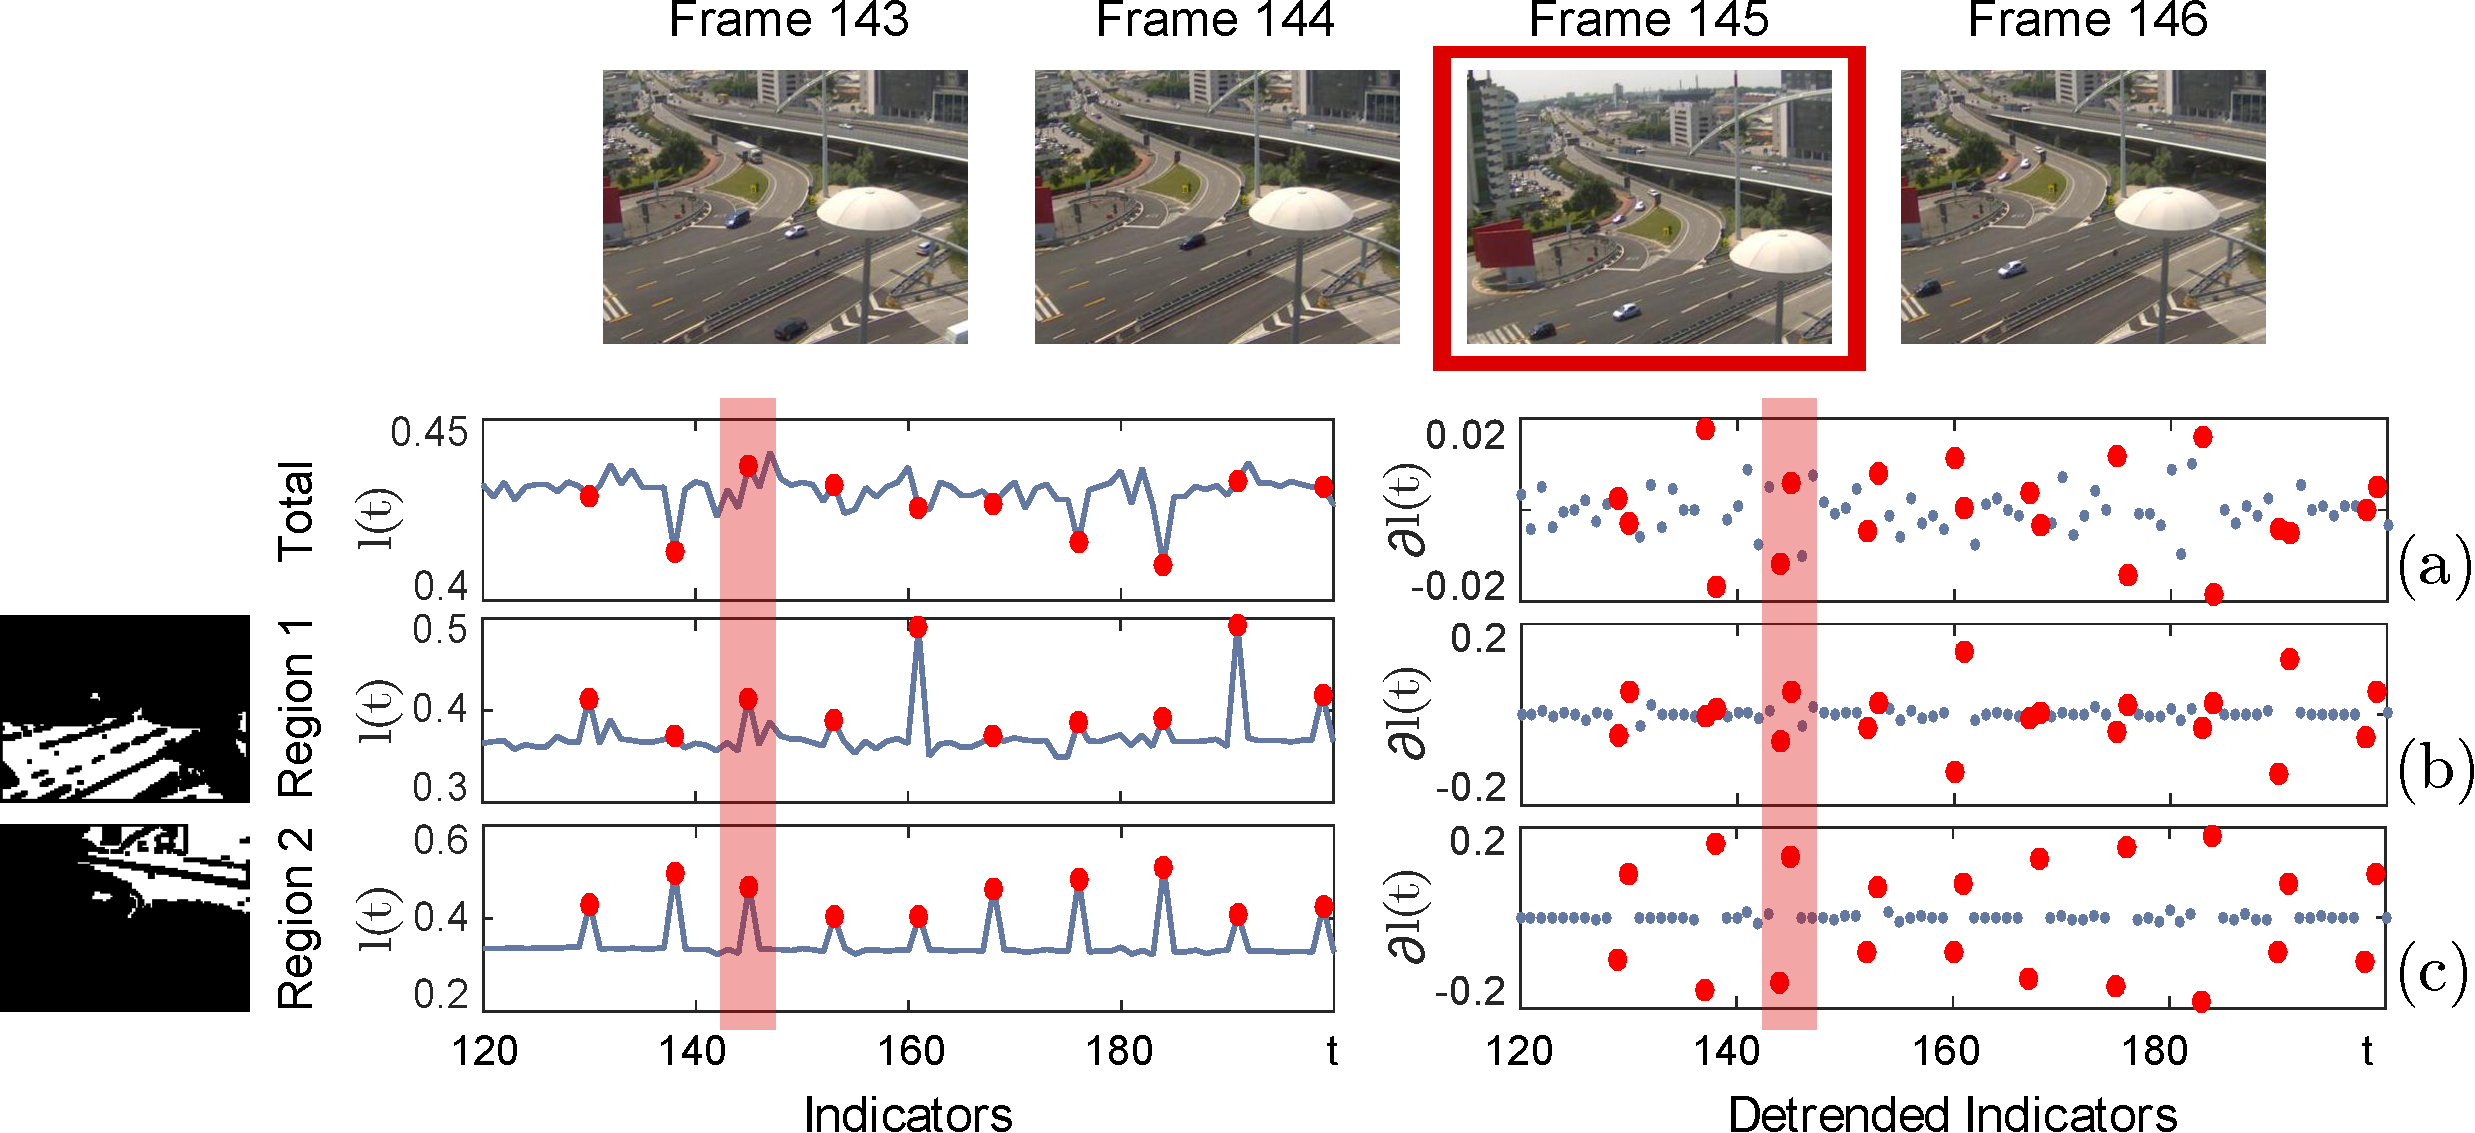
\includegraphics[width=1\linewidth]{Immagini/indicatori}
\caption{Behavior of the average norm of the gradient \textbf{(a)} and its detrending \textbf{(b)} in a sequence with a defocus event.
The tampering event come at $t = 600$.
As illustrated in \textbf{(a)}, even in the case in which there aren't tampering events, there is nonstationarity.
Detrending is done in order to preserve stationarity in normal situations.
Considering the detrending \textbf{(b)} persistent changes become instantaneous:
in particular there is a peak in the instant in which tampering begins.}
\label{fig:indicatori} 
\end{figure}

%Tampering changes the sequence of indicators:
Figure \ref{fig:indicatori}(a) shows how a displacement \gi{TODO} affects the values of $g$. First of all, we observe that displaced frames yield \gi{WHAT} in the indicator sequence. Second, we observe that outlier-detection methods~\cite{Chandola2009} based on density estimates or on confidence intervals --that are very efficient to run-- cannot be straightforwardly applied here, since these are meant for independent and identically distributed (i.i.d.) random variables. In fact, normal changes in the scene or in the illumination yield indicators that follow an unpredictable (but deterministic) trend, beside some high-frequency fluctuations. Therefore, we perform a detrending~\cite{Gustafsson2000} of the indicator sequence by a temporal derivative (line~\ref{DISPL-Test5})
\begin{equation}\label{eq:detrending}
 \partial l_k(t) = l_k(t)-l_k(t-1),  \ \ k = 1, \dots, K\,,
\end{equation}
and we similarly define $\partial g(t)$. 

The sequence of detrended indicators can be suitably monitored by defining the following confidence interval: 
\begin{equation}\label{eq:confidenceRegions}
 [\overline{\partial l}_k(t) - \gamma_l \sigma_{l_k}, \overline{\partial l}_k(t) + \gamma_l \sigma_{l_k}],  k = 1,\dots,K
\end{equation}
where $\overline{\partial l}_k(t)$ denotes the mean and $\sigma_{l_k}$ the standard deviation of $\partial l$ over $R_k$, computed from the tampering-free frames provided for training (i.e. $z_t\,, t = 1, \dots, T_o$) and $\gamma_l >0$ is a tuning parameter. A similar interval is built for $\partial g$ (lines \ref{DISPL-Tr7}). 

During operations, any indicator falling outside its confidence region is considered anomalous (line~\ref{DISPL-Test6}). To raise a camera-displacement alert we require at least $K-1$ indicators $\partial l_k$ to yield an outlier (line~\ref{DISPL-Test8}). This threshold was set to allow a single region not to change, as it typically happens in the sky when the camera is displaced, either horizontally or vertically. In contrast, any outlier in $\partial g$ would yield a blurring\gi{probabilmente e' piu' corretto parlare di blurring invece che defocus.. Adriano, riesci ad allineare? Io menzionerei anche le occlusions assieme al displacement, che dici?} alert (line~\ref{DISPL-Test11}).


It is important to remark that tampering yields outliers in the transient of the detrended indicators~\eqref{eq:detrending}: namely, only the first and last tampered frames correspond to an outlier in the detrended indicators, see Figure~\ref{fig:indicatori}(b). Therefore, detrended indicators have to be monitored in a one-shot manner, targeting the detection of the first-tampered frame. On the one hand, this one-shot solution can increase the detection promptness, and this is particularly important at the low frame-rates we consider. On the other hand, it disregards the fact that tampering might persist over several frames. To take this valuable information into account, some form of sequential monitoring should be applied to the indicator sequence as in~\cite{alippi2010detecting}, and possibly combined with the one-shot monitoring.

\begin{algorithm}[t]
	% \SetAlgoNoLine
	\LinesNumbered
	\SetAlgoNlRelativeSize{0}
	\SetNlSty{small}{}{.}
	\textbf{Input}: $\gamma_l, \gamma_g$, $\{z_t, t = 1, \dots, T_{0}\}$, $\{R_k \ k=1,\dots,K\}$ \\
	\textbf{Configuration}:\\
	\lnl{DISPL-Tr1} Compute $\partial l_k(t)$ and $\partial g(t), t = 1, \cdots, T_o$\\ 
	\lnl{DISPL-Tr7} Compute $\partial l_k$, $\partial g$, $\sigma_{l_k}$ and $\sigma_{g}$.\\
	
	\textbf{Operational phase}:\\
	\lnl{DISPL-Test1} \For{$t=T_{o} + 1,\dots,\infty$}{
		\lnl{DISPL-Test2} Get frame $z_t$, set $n_l =0$;\\
		\lnl{DISPL-Test4} \For{$k=1,\dots,K$}{
			\lnl{DISPL-Test5} Compute $\partial l_k(t)$\\
			\lnl{DISPL-Test6} \If{$\partial l_k(t) < -\gamma_l \sigma_{l_k} \vee \partial l_k(t) > \gamma_l \sigma_{l_k} $}{
				\lnl{DISPL-Test7} $n_l=n_l+1$\\
			}
		}
		\lnl{DISPL-Test8} \If{$n_l\geq K-1$}{
			\lnl{DISPL-Test9} tampering (probably displacement or occlusion) has occurred in $z_t$ \\
		}
		\lnl{DISPL-Test10} Compute $\partial g(t)$\\
		\lnl{DISPL-Test11} \If{$\partial g(t) < -\gamma_g \sigma_{g} \vee \partial l(t) > \gamma_g \sigma_{g} $}{
				\lnl{DISPL-Test9} tampering (probably blurring) has occurred in $z_t$ \\
								}
	}   
	\caption{The Proposed Tampering-Detection Algorithm}
	\label{alg:DISPL}
\end{algorithm}

\subsection{Scene Segmentation}\label{subsec:Segmentation}
Scene has to be preliminarily segmented to define regions  that our algorithm takes as input. To this purpose, we need an external training sequence\gi{Dobbiamo dargli un nome} depicting the scene in its normal conditions without any tampering. Segmentation is performed by associating to each pixel $x\in\mathcal{X}$ a feature vector $\textbf{f}(x)\in \mathbb{R}^5$:
\begin{equation}
\label{eq:featureVector}
\textbf{f}(x)=\left[r(x);c(x);\overline{g}(x);\sigma_{g}(x);\bar{l}(x)\right]\,, \ \forall x \in X
\end{equation}
where $r(x)$ and $c(x)$ represents the row and columns of $x$, $\overline{g}(x)$ and is the gradient norm (smoothed in a neigbhor of $x$) averaged over the training sequence and $\sigma_g$ is the standard deviation of the gradient norm (smoothed in a neigbhor of $x$), computed overtime, and $\bar{l}(x)$ is the average of the gradient over time \gi{ma la deviazione standard della luma nel tempo? cosa faceva?}

Segmentation consists in clustering the feature vectors computed over the whole image by means a weighted version of the k-means algorithm~\cite{han2006data}. In particular, since the components of the feature vector might span very different ranges, the distance between a feature vector and the center of a cluster is measured as the \textit{weighted Minkowski distance}~\cite{de2012minkowski}\gi{.. ho tolto questo, non e' uguale allo standard k-means il resto? from the cluster's centroid is minimum with respect to the distance from the other centroids}, which takes into account the standard deviation of each component for each cluster. 

inside each cluster \cite{kottke1994motion}, in order to consider, during the clustering, also the contribute of the fields which have low variance. \ad{Giacomo: prova a vedere se si capisce cosa voglio dire in queste frasi!!!}

The initial number of clusters is instead chosen by \gi{COME? e poi non ricordo se hai trovato il numero di clusters facendo il k-means con i pesi}

Finally, some canonical morphological image-operations are executed to remove boundaries between different regions, and eventually too small regions. This defines the regions $\{R_k\,, \ k=1,\dots,K\}$.


\subsubsection{Computational Complexity}

The algorithm uses low computational techniques: the biggest effort is made by computation of the feature $g(t)$, which needs $34$ operations per pixel, due to the Sobel filter used during the convolution.
The computational load could be decreased using Fast Fourier Transform (FFT) \cite{brigham1988fast} and operating in the frequency domain.

Segmentation has not been considered because...

FRAME DIFFERENCE:
\begin{equation}
	\label{eq:frameDiffReg}
	\varphi^k(t) = \frac{\sum_{x \in R_k}(z_t(x) - z_{t-1}(x))^2}{|R_k|}, k=1,\dots,K.
\end{equation}
	

%\begin{algorithm}[tp]
%	% \SetAlgoNoLine
%	\LinesNumbered
%	\SetAlgoNlRelativeSize{0}
%	\SetNlSty{small}{}{.}
%	\textbf{Configuration}:\\
%	\lnl{DEF-Tr0} Extract regions $\{R_k\}, k=1,\dots,K$  \\
%	\lnl{DEF-Tr1} \For{$t=1,\dots,T_{o}$}
%	{	\lnl{DEF-Tr2} Acquire frame $z_t$ \\
%		\lnl{DEF-Tr2a} \For{$k=1,\dots,K$}{
%			\lnl{DEF-Tr3a} Compute $g^k(t)$, $\frac{\partial g^k}{\partial t}(t)$ for the region $R_k$\\
%		}
%		\lnl{DEF-Tr3} Compute $g(t)$, $\frac{\partial g}{\partial t}(t)$ \\
%	}
%	\lnl{DEF-Tr6a} \For{$k=1,\dots,K$}{
%		\lnl{DEF-Tr7a} Define thresholds $\Gamma_{min}^k$ and $\Gamma_{max}^k$\\
%	}
%	\lnl{DEF-Tr5} Define CDT parameters on $g(t)$ variance\\
%	\textbf{Operational phase}:\\
%	\lnl{DEF-Test1} \For{$t=T_{o},\dots,\infty$}{
%		\lnl{DEF-Test2} Acquire frame $z_t$ \\
%		\lnl{DEF-Tr3b} Compute $g(t)$, $\frac{\partial g}{\partial t}(t)$ \\
%		\lnl{DEF-Test2a} $n=0$\\
%		\lnl{DEF-Test4a} \For{$k=1,\dots,K$}{
%			\lnl{DEF-Test5a} Compute $g^k(t)$, $\frac{\partial g^k}{\partial t}(t)$ for the region $R_k$\\
%			\lnl{DEF-Test6a} \If{$\frac{\partial g^k}{\partial t}(t) < \Gamma_{min}^k \vee \frac{\partial g^k}{\partial t}(t) > \Gamma_{max}^k $}{
%				\lnl{DEF-Test7a} $n=n+1$\\
%			}
%		}
%		\lnl{DEF-Test81} \If{$n \geq K-1$}{
%			\lnl{DEF-Test91} $z_t$ is a defocused frame\\
%		}
%		\lnl{DEF-Test8} \If{CDT detect a change on $g(t)$ variance}{
%			\lnl{DEF-Test9} $z_t$ is a defocused frame\\
%		}
%	}   
%	\caption{Blur detection algorithm}
%	\label{alg:DEFOCUS}
%\end{algorithm}

%\gi{Adriano: inserisci qui l'algoritmo e traducilo in inglese. Se riusciamo lo spostiamo prima di tutte le sottosezioni}

\section{Experiments}\label{sec:experiments}
\gi{Per ultimo: The proposed algorithm has been implemented in MATLAB, }

Experiments are meant to show the effectiveness of the proposed algorithm on real-world sequences, and in particular on assessing the advantages of using segmentation for detecting camera displacements.

We have acquired two datasets to test our method. The first dataset contains \gi{how many?} sequences taken from webcams recording urban areas (as in Figure \ref{fig:sequences}(a)), where we have synthetically introduced blurring by means of a gaussian filters (Figure \ref{fig:sequences}(b)), and displacement by concatenating frames from sequences depicting similar environments (Figure \ref{fig:sequences}(c)). In some cases, sequences contained real tampering events, as in Figure \ref{fig:sequences}(d).\\
\begin{figure}[t]
\centering
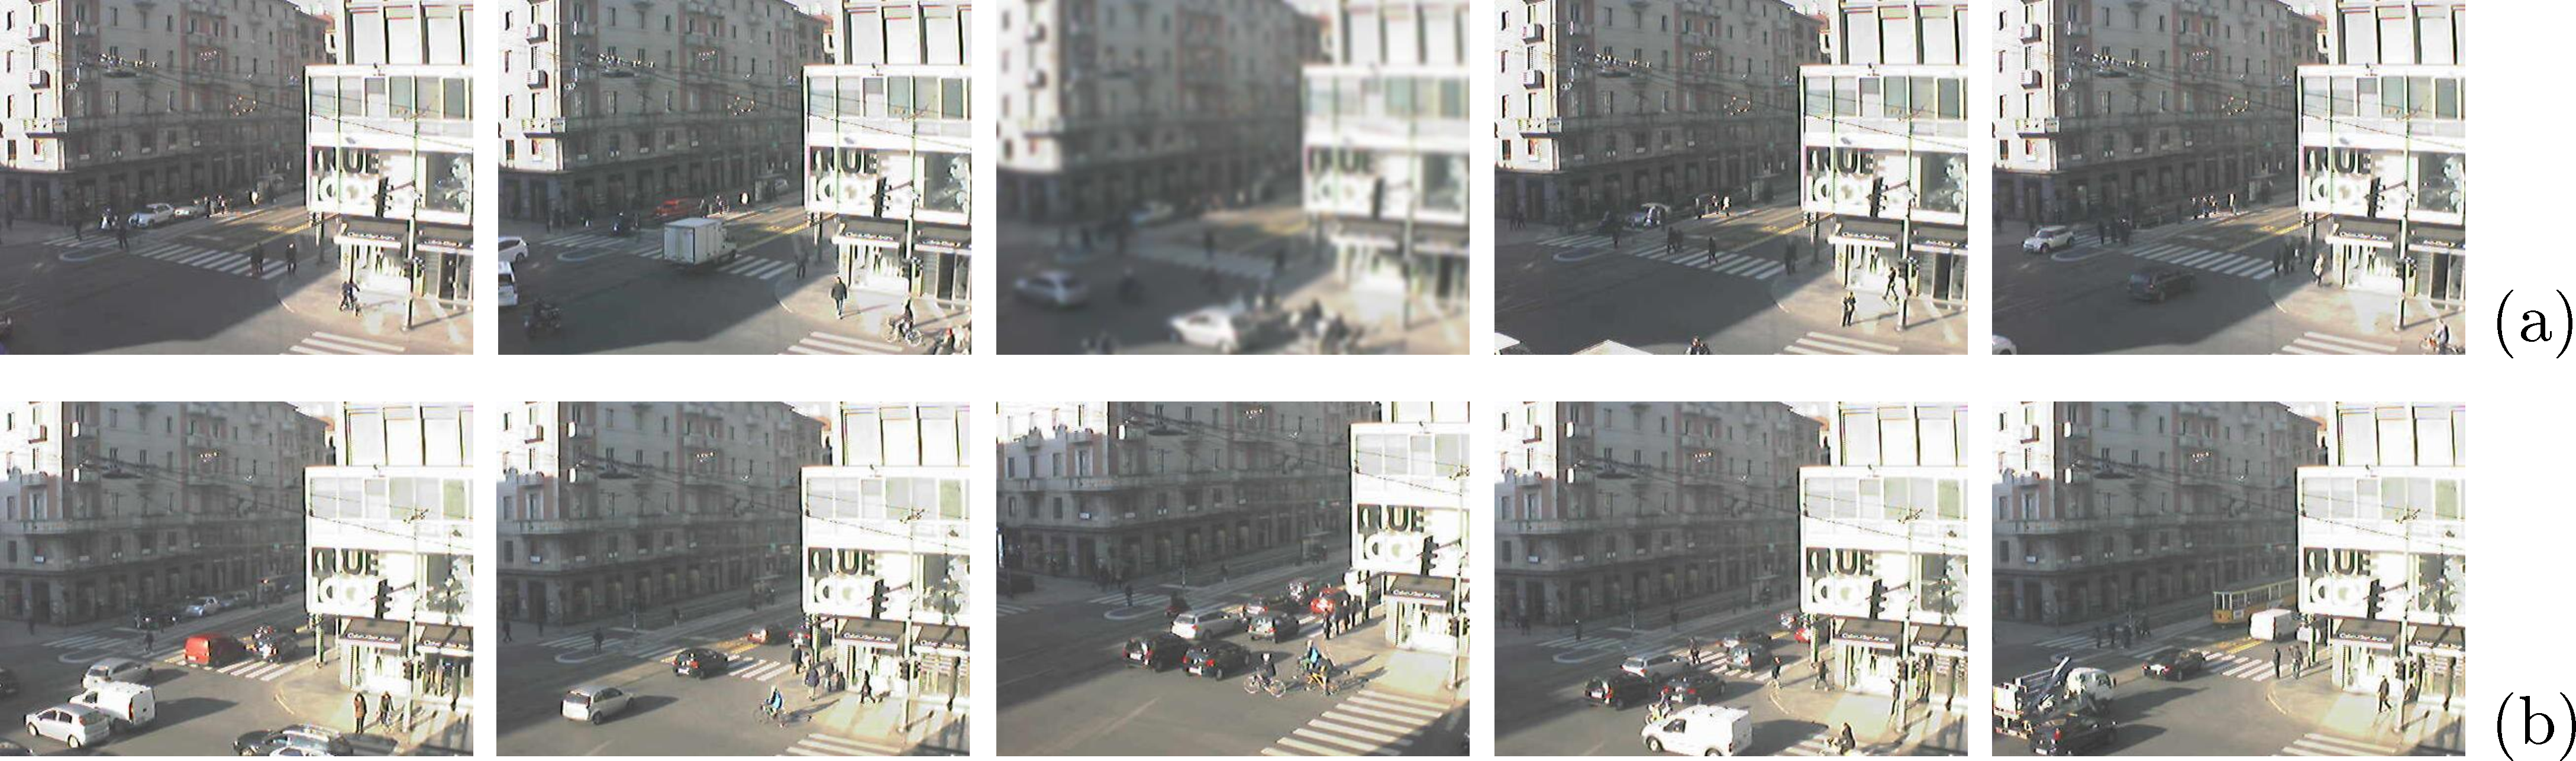
\includegraphics[width=1\linewidth]{Immagini/sequenze}
\caption{Sequences taken from webcams: \textbf{(a)} no tampering events; \textbf{(b)} defocus event on 4-th and 5-th frames, created using gaussian filtering; \textbf{(c)} displacement event on 4-th and 5-th frames, created using concatenation between similar sequences; \textbf{(d)} real displacement event on 4-th frame.}
\label{fig:sequences}
\end{figure}
The second dataset was recorded using a Raspberry Pi Model B+, with its camera module, and the tampering was introduced by moving the device or spraying water on the camera len.\gi{una footnote dicendo sequences can be released upon request?}

Typical figures of merit for one-shot monitoring methods have been used to assess the performance of the proposed algorithm. In particular we compute the ROC curves varying $\gamma_l$ and $\gamma_g$ in a range of values. ROC curve reports :
\[1-\text{SPECIFICITY}_\gamma = 1-\frac{\text{TN}_\gamma}{\text{TN}_\gamma+\text{FP}_\gamma}=\frac{\text{FP}_\gamma}{\text{TN}_\gamma+\text{FP}_\gamma},\]
while on th y-axis there is:
\[\text{RECALL}_\gamma=\frac{\text{TP}_\gamma}{\text{TP}_\gamma+\text{FN}_\gamma}.\]
The construction of these curves permits us to make a comparison with respect to other methods.\gi{io le metterei solo in una equazione entrambe, e per 1-specificity solo la terza formula}

\begin{description}
	\item[TP]  True positives. It measures the number of tampering events correctly detected by the algorithm.\\ 
	\item[TN]  True negatives. It measures the number of frames without tampering that are not detected by the algorithm. \\ 
	\item[FP]  False positives. It measures the number of tampering events erroneously detected by the algorithm.\\ 
	\item[FN]  False negatives. It measures the number of tampering events not detected by the algorithm. \\ 
\end{description} 
\gi{questo lo metterei solo nel testo sotto le formule sopra}

\gi{io inizierei dai metodi con cui confrontarci}
In particular the alternative approaches that we have considered working:
\begin{itemize}
\item considering the whole scene for the features computation;
\item considering adaptive region, as described in Section \ref{sec:propSol}, for the feature computation;
\item considering voronoi regions \cite{aurenhammer1991voronoi}, which are easier to compute with respect to our solution but don't consider the scene content, for the feature computation.
\end{itemize}

FRAME DIFFERENCE:
\begin{equation}
	\label{eq:frameDiffReg}
	\varphi^k(t) = \frac{\sum_{x \in R_k}(z_t(x) - z_{t-1}(x))^2}{|R_k|}, k=1,\dots,K.
\end{equation}

%
%% \subsection{Alternative Approaches}\label{subsec:AlternativeApproaches}
%
%
%\subsection{Performance Assessment}
%\gi{Adriano: Dire come vengono calcolate le ROC curves TPR e FPR, le cifre di merito insomma, spiegando bene che parametro varia}
%
%\gi{Adriano: metti entrambe le ROC curves, affiancate e per bene ed alcuni esempi di sequenze}
\begin{figure}[t]
\centering
\subfigure[]{\label{fig:ROCdisplacement}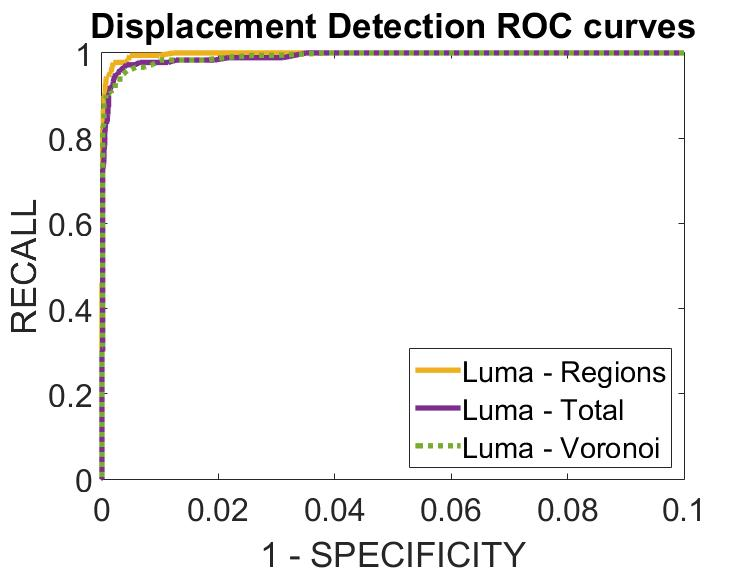
\includegraphics[width=0.45\linewidth]{Immagini/ROCdisplacement}}
\subfigure[]{\label{fig:ROCdefocus} 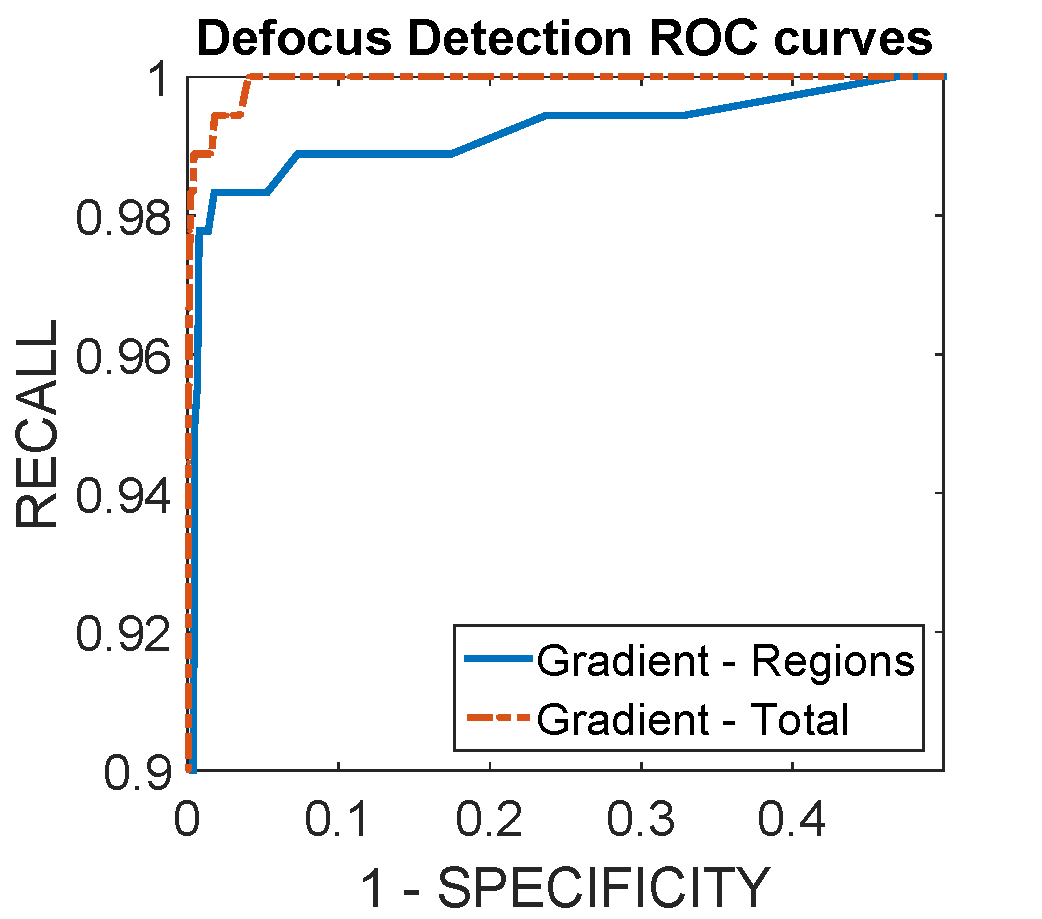
\includegraphics[width=0.45\linewidth]{Immagini/ROCdefocus}}
\caption{ROC curves for displacement detection, considering three alternative approaches. \textbf{(a)} Analysis of the mean luma energy. \textbf{(b)} Analysis of the frame differencing.}
\label{fig:ROC}
\end{figure}
%\begin{figure}[htb]
%\centering
%\subfigure[]{\label{fig:buenosAiresDef}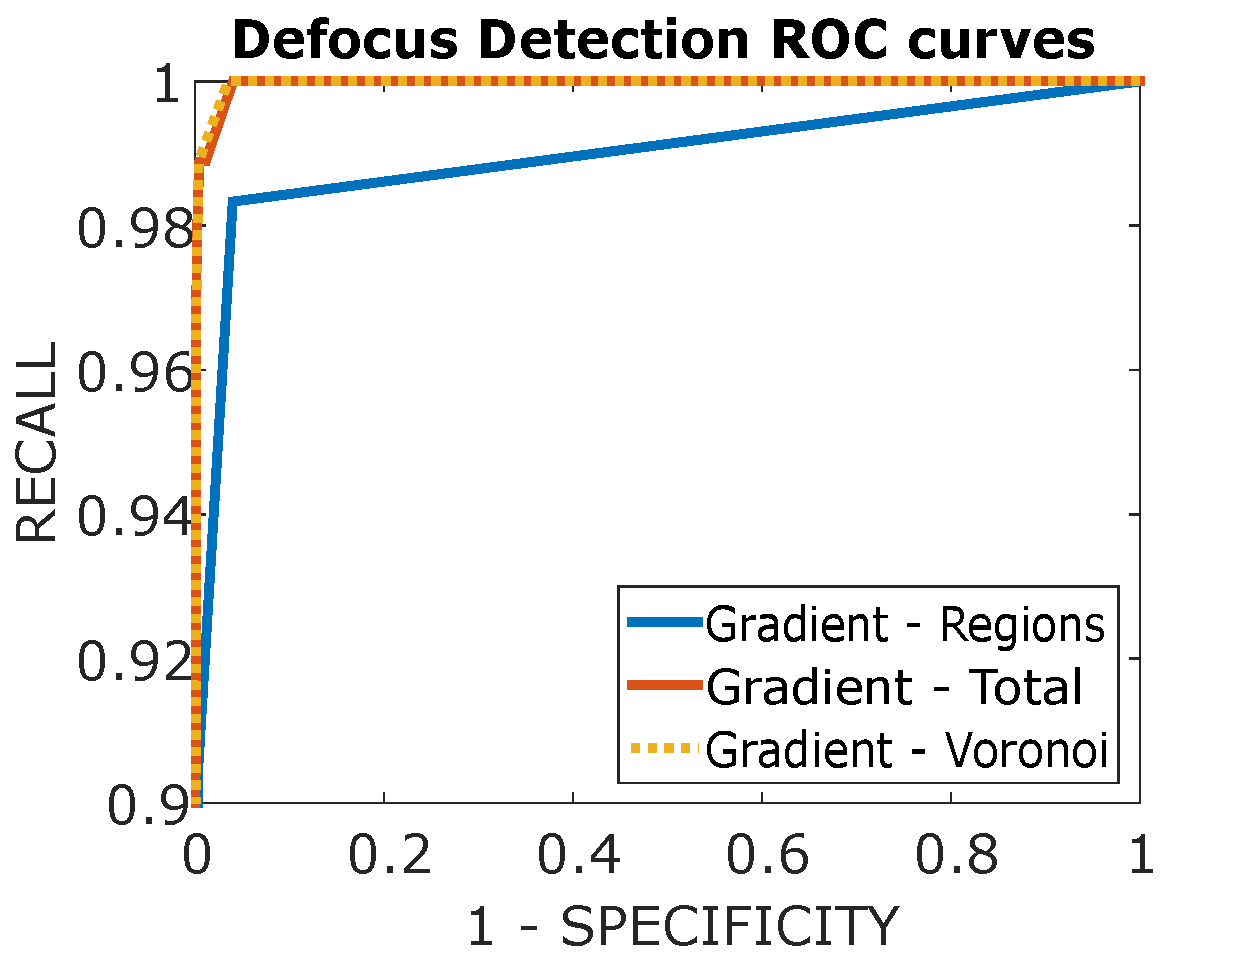
\includegraphics[width=0.45\linewidth]{Immagini/ROCdefocus1}}
%\subfigure[]{\label{fig:buenosAiresDispl} 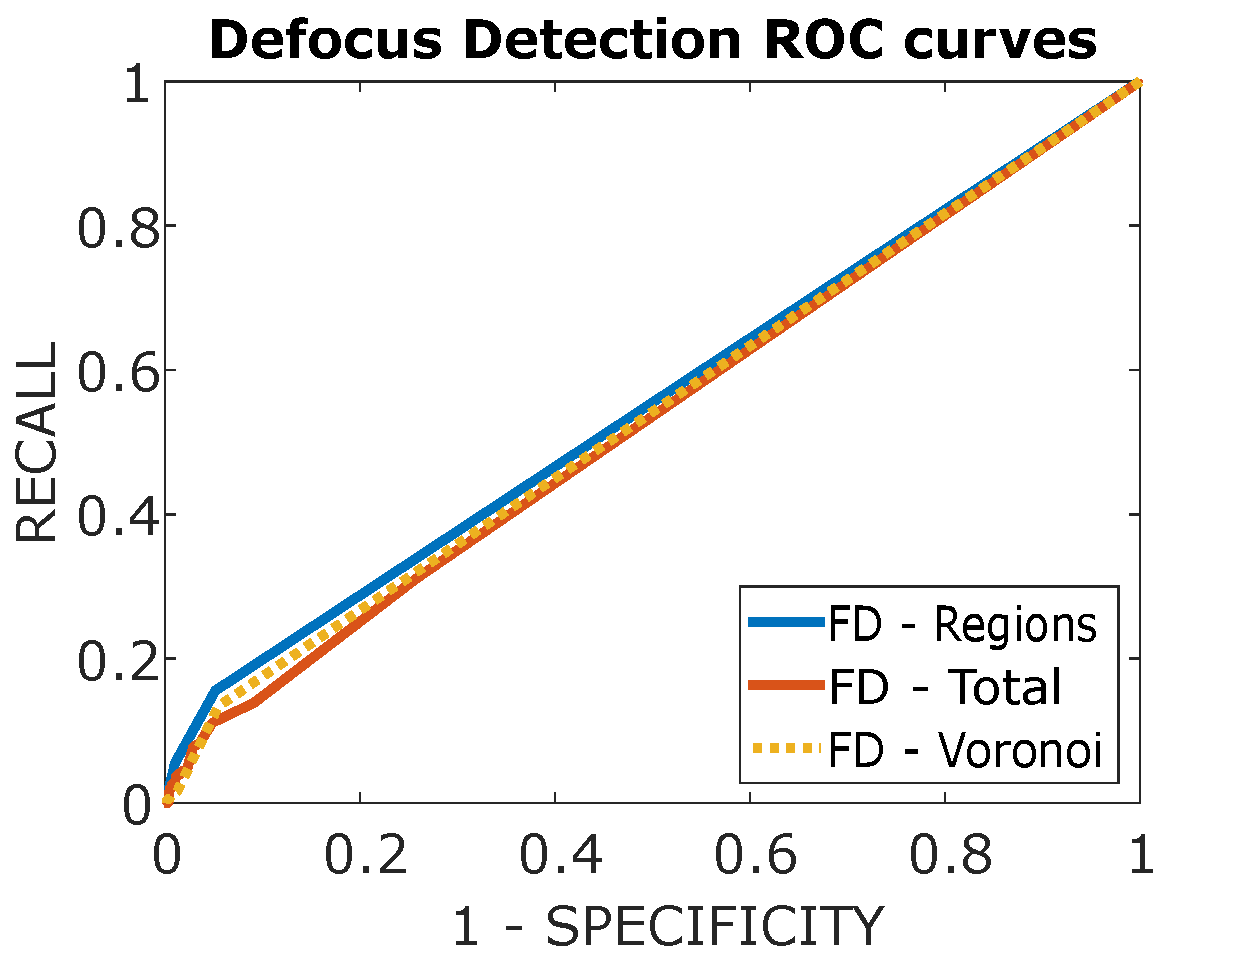
\includegraphics[width=0.45\linewidth]{Immagini/ROCdefocus_fd}}
%\caption{ROC curves for defocus detection, considering three alternative approaches. \textbf{(a)} Analysis of the mean gradient energy. \textbf{(b)} Analysis of the frame differencing.}
%\label{fig:ROCdisplacement}
%\label{fig:ROCdefocus}
%\end{figure}
Experimental results are shown in Figures \ref{fig:ROCdisplacement} and \ref{fig:ROCdefocus}.
As we could see there is an improvement, in the detection of camera displacements, with our approach which separately analizes the behavior of indicators in adaptive regions.
On the other side, as illustrated in Figure \ref{fig:ROCdefocus}, when monitoring indicators meant to detect blur/defocus, it is more convenient to consider the whole scene at once.

\begin{table}[tbh]
\centering
\begin{tabular}{l|l|l|l|l|l|l|}
\cline{2-7}
& \multicolumn{3}{l|}{\cellcolor[HTML]{C0C0C0}\textbf{Displacement Detection}}  & \multicolumn{3}{l|}{\cellcolor[HTML]{C0C0C0}\textbf{Defocus Detection}} \\ \cline{2-7} 
& \cellcolor[HTML]{EFEFEF}\textbf{Regions} & \cellcolor[HTML]{EFEFEF}\textbf{Total} & \cellcolor[HTML]{EFEFEF}\textbf{Voronoi} & \cellcolor[HTML]{EFEFEF}\textbf{Regions} & \cellcolor[HTML]{EFEFEF}\textbf{Total} & \cellcolor[HTML]{EFEFEF}\textbf{Voronoi} \\ \hline
\multicolumn{1}{|l|}{\cellcolor[HTML]{EFEFEF}\textbf{Luma}}     & 0.9994 & 0.9989 & 0.9985  &            &            &             \\ \hline
\multicolumn{1}{|l|}{\cellcolor[HTML]{EFEFEF}\textbf{Gradient}} &  		 &  		  &             & 0.9895 & 0.9996 & 0.9996  \\ \hline
\multicolumn{1}{|l|}{\cellcolor[HTML]{EFEFEF}\textbf{FD}}         & 0.9974 & 0.9944 & 0.9974  & 0.5526 & 0.5322 & 0.5391  \\ \hline
\end{tabular}
\caption{Area under curve of the analized solutions}
\label{tab:AUC}
\end{table}

%Numero di operazioni richieste:
%Calcolo di g(t):
%\begin{itemize}
%\item Norma gradiente: 34 FLOP per pixel
%\item Media delle norme del gradiente
%\end{itemize}
%Calcolo di l(t):
%\begin{itemize}
%\item Media dei valori di grigio
%\item Detrending: 1 FLOP per frame
%\end{itemize}
%Monitoraggio one-shot: 2 confronti
%Monitoraggio sequenziale: 
%Ogni 20 frame
%Calcolo intervalli di confidenza: ~70 FLOP
%Confronto tra intervalli di confidenza: 2 confronti



\section{Conclusion}\label{sec:Conclusion}
\gi{Adriano: butta in inglese gli ongoing works (come ultima cosa)}
.

Random Toughs:
\begin{itemize}
\item The problem of false alarms, radio module activation
\item Other tampering attacks like obfuscation (??) which might be due to environmental phenomena such as rain, fog and mist over the camera lenses have to be detected by image analysis methods
\item Displacement can be perceived by MEMS as well but these device alone are prone to false alarms. Visual inspection is necessary to reduce false alarms
\end{itemize}
Ongoing work regards the extension of our solution to other types of tampering, as occlusions or imaging sensor degradations.
Furthermore, we are investigating strategies to improve the detection performance and reduce the number of \textit{FP}s by combination of our solution with other techniques:
for example we could use sequential techniques on the features, or integrate the frame analysis with the data extracted from MEMS inertial sensors.   

\section*{Acknowledgments}\label{sec:Acknowledgments}
Authors would like to thank ST for supporting Adriano Gaibotti.

\bibliographystyle{unsrt}
\bibliography{bibl_tesi}

%\begin{thebibliography}{1}
%	
%	\bibitem{Einstein}
%	A. Einstein, On the movement of small particles suspended in stationary liquids required by the molecular-kinetic theory of heat, Annalen der Physik 17, pp. 549-560, 1905.
%	
%\end{thebibliography}
\end{document}



%
%
%
\subsection{Indicators}\label{subsec:Indicators}

%\begin{equation}
%\label{eq:gradientRegions}
%\begin{array}{ccc}
%g^k(t)&  = & \mathcal{G}^k[z_t] = \frac{\sum_{R_k}\| \nabla z_t(x) \| _2^2 }{|{R_k}|}\\
%\partial g^k(t) & =& g^k(t)-g^k(t-1) 
%\end{array},
%\end{equation}
%
%In particolare, per il calcolo delle derivate orizzontali  abbiamo utilizzato il seguente filtro $f_h$:
%\[f_h = f \circledast \left[ \begin{array}{rcl}
%1 & 0 & -1
%\end{array}\right], \] 
%mentre per il calcolo delle derivate verticali abbiamo utilizzato il seguente filtro $f_v$:
%\[f_v = f \circledast \left[ \begin{array}{r}
%1 \\ 0 \\ -1
%\end{array}\right], \]
%dove abbiamo indicato con $\circledast$ l'operatore di convoluzione.
%Il filtro $f$, invece, \`e ottenuto tramite un campionamento della \textit{funzione gaussiana} $h$, con media $0$ e deviazione standard $\sigma$
%\begin{equation}
%\label{eq:gaussian}
%h(i,j)=\frac{1}{2\pi\sigma^2}\exp\left(-\frac{i^2+j^2}{2\sigma^2}\right),
%\end{equation}
%e ponendo il valore massimo di questa funzione nel centro del filtro.
%Con questi filtri \`e possibile calcolare la \textit{norma del gradiente} nel seguente modo:
%
%Una volta calcolata la norma del gradiente \`e possibile farne la media come specificato in \eqref{eq:energyGradient}.
%Il risultato finale \`e un indicatore \textit{scalare} per ciascun frame acquisito, che pu\`o essere monitorato per individuare eventi di sfocature. 
%In particolare ci aspettiamo che l'evento di sfocatura provochi un abbattimento del valore di $g$.